\subsection{Opalinus Claystone from Mont-Terri, Switzerland}

\Authors{Tilo Kneuker, Bernhard Vowinckel, Gesa Ziefle, Jobst Maßmann (BGR)}

\subsubsection{The Mont Terri Rock laboratory}\label{sec:mont_terri}

Opalinus claystone is a very promising hostrock for the safe disposal of heat emitting nuclear waste. This type of hostrock has been investigated in the Mont Terri Rock laboratory for more than 24 years. The Mont Terri rock laboratory is a facility to conduct research in the deep geological underground at in-situ scale, such as the safe deposition of radioactive waste, where the local host rock is Opalinus Clay. The rock laboratory is located within the Jura Mountain fold belt. The development of the Jura fold belt began in the Middle Miocene around 12 million years ago, which was constrained by the first occurrence of overthrusted and folded molasse sediments \cite{bolliger1993}. The overthrust of the frontal fold and thrust belt over the allochthonous foreland (Tabular Jura) occurred ca. 10.5 million years ago \cite{becker2000}. More specifically, the Mont Terri rock laboratory is located in the southeast dipping fold limb of the NW-vergent Mont Terri anticline \cite{nussbaum2011}. The total amount of shortening of the anticlinal structure is approximately 2.1 km \cite{freivogel2003}. During the folding process, the northwestern fold limb of the Mont Terri anticlinal structure was sheared-off and now lies on top of the Tabular Jura (Figure \ref{fig:bgr_mt_sideview}). The Mont Terri anticlinal structure developed in a special structural setting at the intersection between the frontal part of the Jura fold belt (main shortening direction NW-SE) and the roughly N-S oriented structural elements of the Rhine-Bresse-graben transfer zone \cite{nussbaum2011}.

\begin{figure}[!ht]
\centering
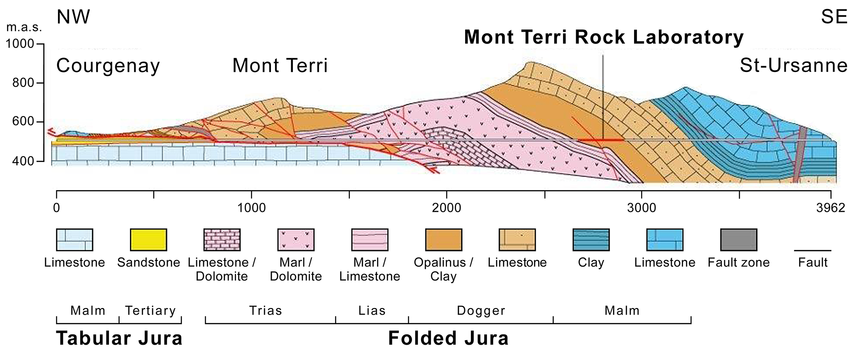
\includegraphics[width=1\textwidth]{./figures/bgr_mont_terri_side_view.png}
\caption{Geological cross section along the motorway tunnel through the Mont Terri anticline. From: Kaufhold et al. (2016) \cite{kaufhold2016}, based on Freivogel \& Huggenberger (2003) \cite{freivogel2003}.}
\label{fig:bgr_mt_sideview}
\end{figure}

The Mont Terri rock laboratory branches off from the security gallery of the motorway tunnel near the town of St. Ursanne (NW Switzerland). The rock laboratory is located entirely within the Middle Jurassic Opalinus Clay formation. The thickness of the Opalinus Clay in the rock laboratory is around 130 m \cite{hostettler2018} and the layers are dipping with ca. 40° towards SE. The depth below ground varies between 230 m and 320 m, depending on the topography \cite{heitzmann2001}. Since 1996, a total of 1400 m of galleries and niches have been excavated in the Mont Terri rock laboratory (Figure \ref{fig:bgr_mt_topview}). The Mont Terri rock laboratory is a generic scientific research laboratory. At Mont Terri, there will be no storage of radioactive waste.

\begin{figure}[!ht]
\centering
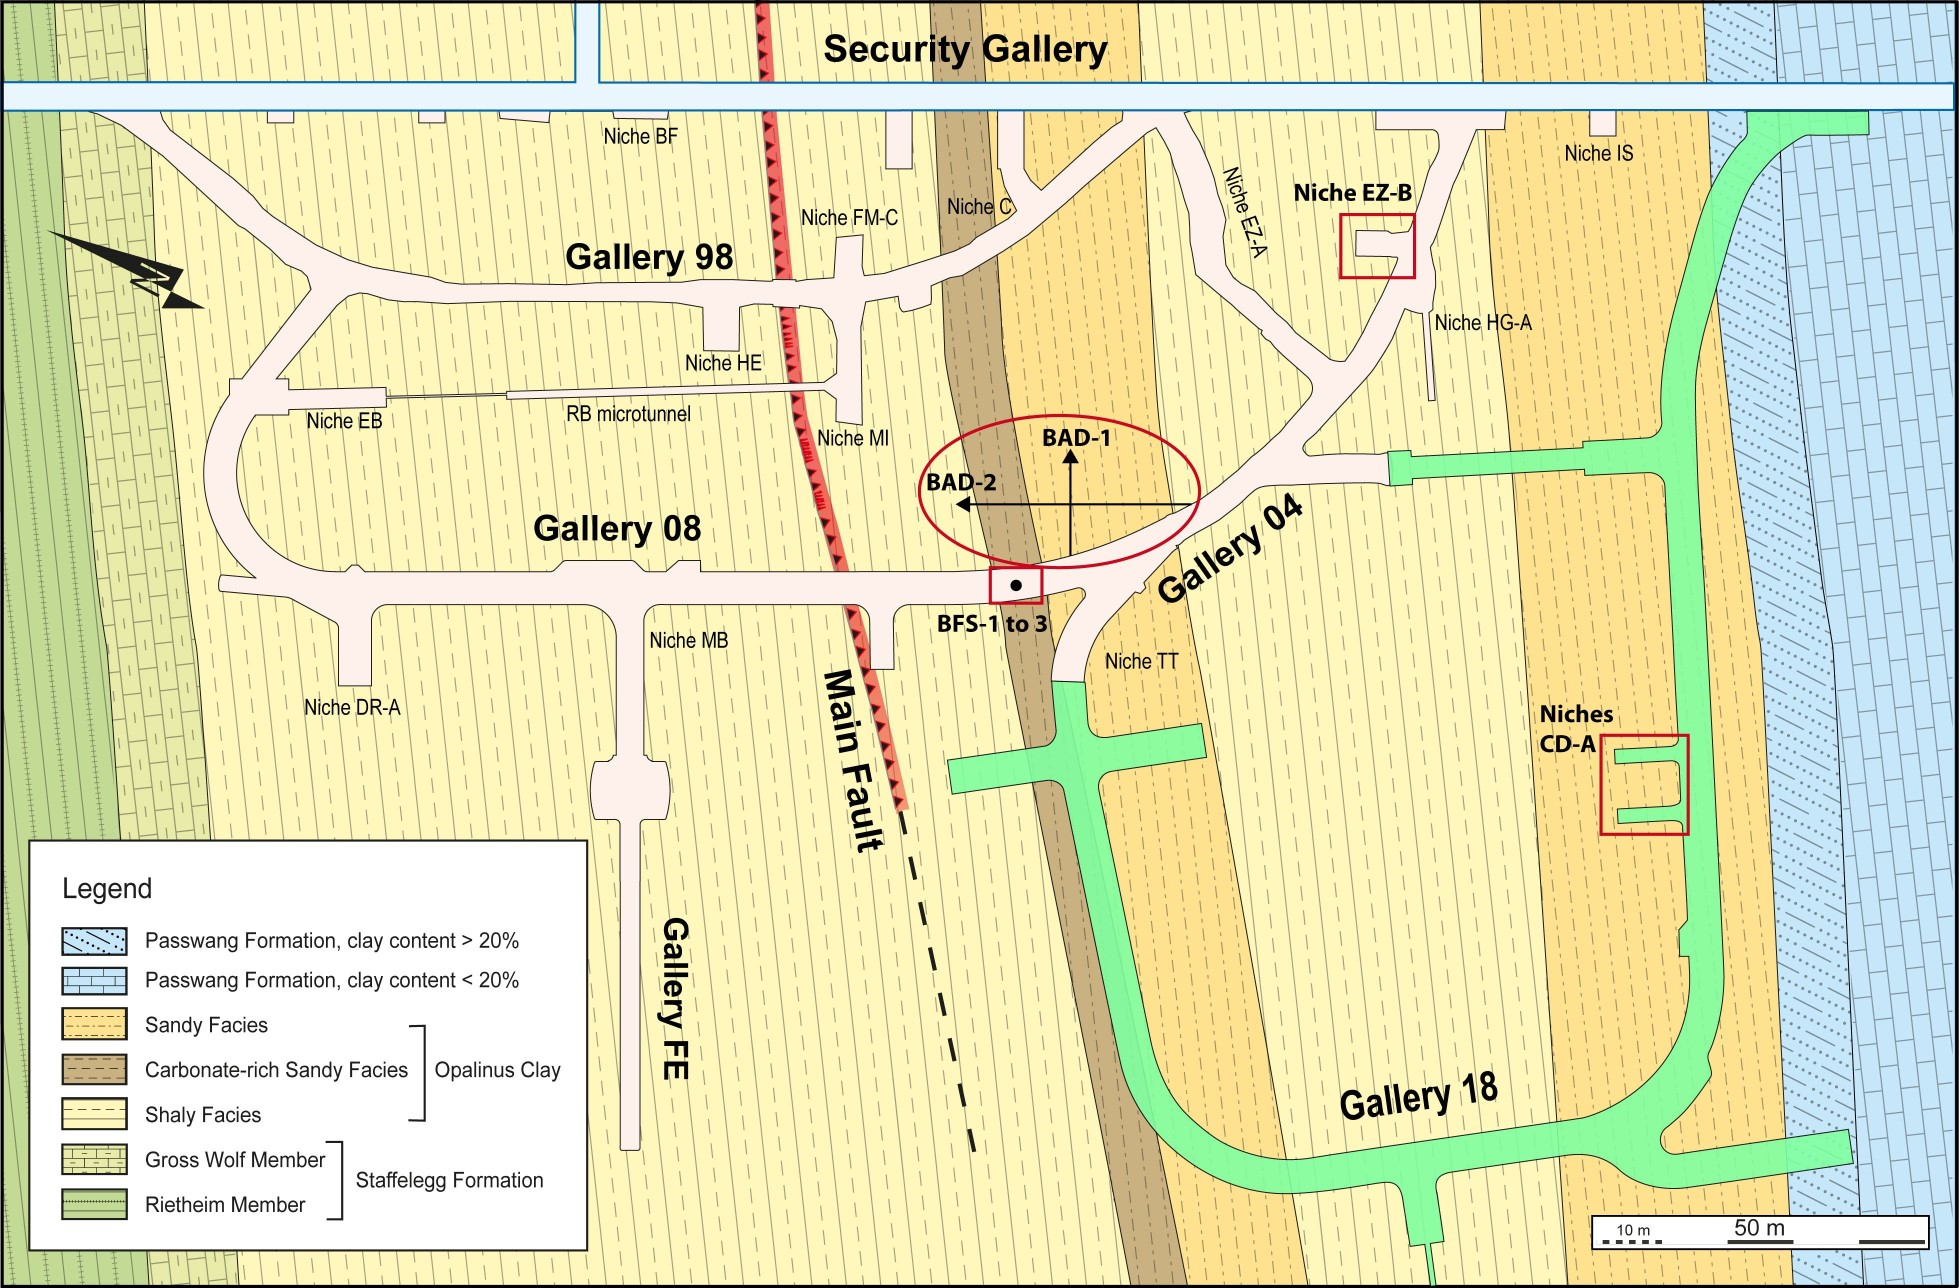
\includegraphics[width=1\textwidth]{./figures/bgr_mont_terri_top_view.jpg}
\caption{Geological map of the rock laboratory with all in-situ experiments relevant for the GeomInt project including the locations of the two AD-boreholes (BAD-1, BAD-2), the drilling for the FS-experiment (BFS-1 to 3), the EZ-B niche for the CD/LP experiment and its successor experiment CD-A in Gallery 18. The different facies types of the Opalinus Clay can be recognized by the different shades of brown and yellow (map modified from Mont Terri Consortium, swisstopo).}
\label{fig:bgr_mt_topview}
\end{figure}

The Opalinus Clay in the rock laboratory is composed of a dark gray claystone that was named after the ammonite species Leioceras opalinum. This claystone formation was deposited during the period of the Toarcian/Aalenian, at an age of approximately 174 million years. The Opalinus Clay is exposed along the rim of the Swabian and Franconian Alp in Germany and stretches into northern Switzerland \cite{einsele1983}. The Opalinus Clay was deposited in a shallow-marine, epicontinental milieu in the area of the storm wave base at approximately 20 m to 50 m water depth \cite{wetzel2003}. Coarser siliciclastic components are of detritical origin. Potential sources for the detritic components are the areas of the Bohemian Massif and the Vindelician Landmass \cite{wetzel2003}. During Cretaceous burial, the Opalinus Clay experienced maximum palaeo temperatures of $75^{\circ}$~C to $90^{\circ}$~C \cite{bossart2008} at a maximum burial depth of 1.35 km. The Opalinus Clay at the Mont Terri site is underlain by  marls of Upper Toarcian age and overlain by limestones (Bajocian), some of which act as karst aquifer \cite{pearson2003}.

The Opalinus Clay at the Mont Terri rock laboratory can be subdivided into three main facies types \cite{bossart2008}. First, the shaly facies occupies the largest area of the rock laboratory (Figure \ref{fig:bgr_mt_topview}). It dominates the lower part of the Opalinus Clay formation. It consists of mica-bearing clay and marly shales as well as flasery, marly layers characterized by bioturbation. The clay-rich facies occurring in the upper part of the profile contains a higher volumetric content of quartz grains. Second, the sandy facies occurs in the middle and upper part of the profile (lower and upper sandy facies). It includes medium gray marly claystones with intercalated, bioturbated marly layers or lenticular, gray sandy limestones and pale sand layers of approximately 1-10 mm thickness that include pyrite as well. Third, a carbonate-rich sandy facies of 5 m thickness occurs in the middle part of the rock formation. It consists of calcareous sandstones with intercalated bioturbated limestone layers, which show a relatively high proportion of detritic quartz and white mica. The different facies types of the Opalinus Clay can be attributed to varying sedimentation conditions in a shallow marine environment (like variations in depth and current directions). The carbonate-rich facies is typical for the Jura region in western Switzerland and it doe not occure in the siting regions.

The mineralogical composition of the Opalinus Clay was examined by Traber \& Blaser (2013) \cite{traber2013} for several locations in northern Switzerland. For the clay-rich facies, the clay mineral content varies between 40 wt\% and 75 wt\%. The clay minerals determined by Traber \& Blaser (2013) \cite{traber2013} include illite, kaolinite and smectite-illite mixed layer minerals. According to Traber \& Blaser (2013) \cite{traber2013}, the proportion of swellable clay minerals is around 10 wt\%. Detritic components such as quartz and feldspars typically make up to 20 wt\% of the investigated samples. The carbonate content (calcite and dolomite) is around 20 wt\%. The sandy facies of the Opalinus Clay is composed of up to 40 wt\% clay minerals and ca. 30 wt\% quartz; it shows a lower amount of clay minerals in favor of a higher quartz content, compared to the shaly facies \cite{heitzmann2001}. 

The BGR has been involved in a number of campaigns to study in-situ conditions of clay rock, of which the following four are particularly noteworthy within the context of the GeomInt-Project. First, the CD/LP experiment investigates the long-term cyclic deformation (CD) due to seasonally induced cyclic swelling and shrinkage in a niche of the rock laboratory. In addition, a follow-up project, the CD-A experiment, has been prepared in recent years, to distinguish between deformation processes due to stress redistribution and seasonal variations in air humidity that cause saturation (swelling) and desaturation (shrinkage) of the rock and stress redistribution alone. To this end, two identical niches were excavated, one sealed towards the gallery and with a high humidity inside to minimize desaturation and one open to the general air circulation of the rock laboratory. The measurement campaign was started in October 2019 \cite{ziefle2019}. Third, the AD-experiment intends to provide an improved process understanding for the experimental-numerical analysis of discontinuities. Finally, the Fault Slip (FS) – experiment addresses the fault reactivation due to pressure-induced percolation in a low-permeability, large-scale discontinuity in the Mont Terri rock laboratory. The AD is directly relevant to the numerical and experimental investigations presented in Sections \ref{sec:mex05} - \ref{sec:mex12}, because the rock material used in these experiments were drilling samples from this experiment. Hence, we provide a brief overview for the campaign in the following. 

\subsubsection{The CD/LP Experiment in the Mont Terri Rock laboratory}

The Mont Terri Rock laboratory in Switzerland hosts a multitude of in-situ experiments that investigate the response of Opalinus claystone to various geotechnical applications. An overview of the rock laboratory is given in Section \ref{sec:mont_terri}. In particular, the CD (Cyclic Deformation) experiment has been a valuable site to gather experimental data at the in-situ scale to investigate the hydraulic-mechanial coupling induced by swelling and shrinking of Opalinus claystone due to cyclic variations of air humidity. Section \ref{sec:mex10} focuses on the numerical investigation of these processes. Here, we provide a brief overview of the experimental CD campaign at the Mont Terri Rock Laboratory. 

The experiment itself is located in the EZ-B niche (Figure \ref{fig:bgr_mt_topview}). The experiment has been conducted for more than 13 years to provide information on the swelling and shrinkage behavior of Opalinus Clay in the Mont Terri rock laboratory. The idea was to analyze a niche that is not covered by shotcrete. Instead, the clay rock remains in direct contact with the atmospheric conditions of the main gallery for the entire time. Consequently, the swelling and shrinkage is induced by changes in temperature and relative humidity, which can decrease to values as low as 65\% in the winter and reaches values of up to 100\% in the summer. 

\begin{figure}[!ht]
\centering
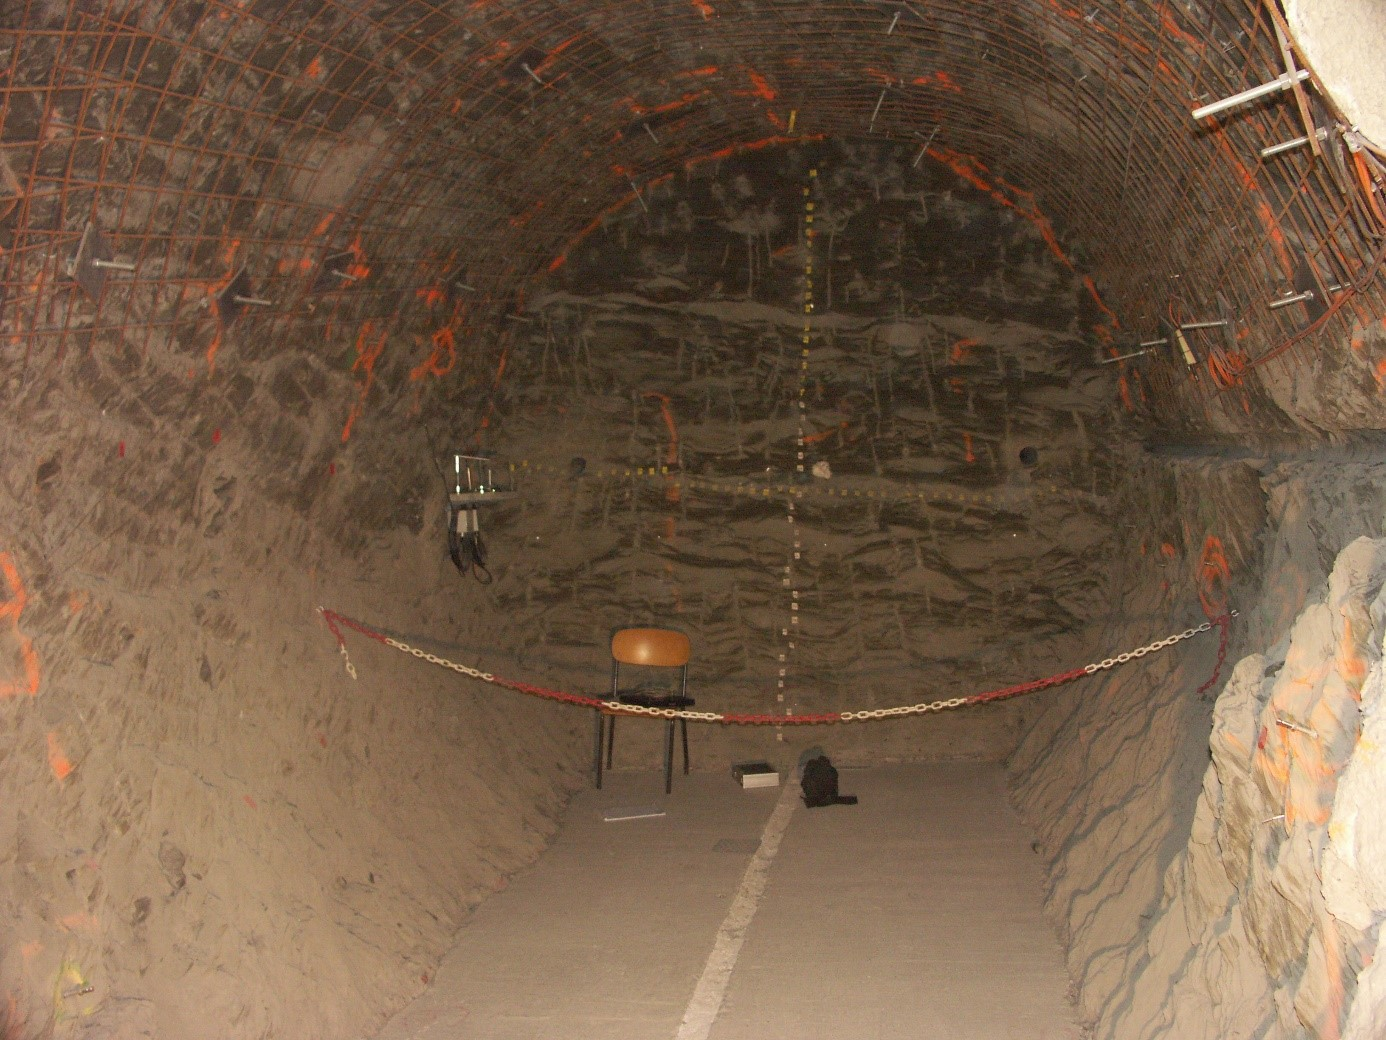
\includegraphics[width=1\textwidth]{./figures/bgr_CD_experiment.jpg}
\caption{The EZ-B niche in the Mont Terri rock laboratory, where the CD/LP experiment has been conducted since 2006 (photo: Mont Terri consortium, swisstopo).}
\label{fig:bgr_CD_experiment}
\end{figure}

A special focus of this experiment was to investigate the long-term impact of these seasonal variations on the temporal evolution of the cracks that occur during the excavation process and make up the Excavation Damaged Zone (EDZ). To this end, the EZ-B niche was excavated in the years 2004/2005 (Figure \ref{fig:bgr_CD_experiment}). Subsequently, the niche was equipped with a comprehensive set of measurement devices to record the evolution of temperature, water content, convergence of the niche and crack development at the tunnel walls over time. This measurement campaign was started in 2006 and has been continued until today to investigate long-term effects. Note that the experiment was transferred into the LP-A experiment to explicitly focus on the long-term monitoring of pore pressure. The CD/LP experiment under in-situ conditions was supplemented by laboratory experiments with drill cores to determine hydraulic-mechanical properties of the clay rock, such as porosity, grain density, etc. \cite{matray2013}. 

Characteristic macroscopic cracks on the tunnel walls have been monitored and the field data of the crack opening show a good correlation with the seasonal variation of temperature and humidity. The cyclic deformation of the crack opening yields a re-occurring compression perpendicular to the crack during summer, which typically is a time of high relative humidity and, hence, the swelling causes an increase of rock volume \cite{jaeggi2012}. This characteristic behavior of swelling and shrinking was successfully reproduced by means of hydraulic-mechanically coupled numerical simulations \cite{ziefle2018}, which provides valuable benchmark data for future investigations of the cyclic deformation of clay rock.

\subsubsection{The AD-Experiment}

The aim of the experiment is to provide core samples from the sandy facies of the Opalinus Clay as a typical example of an argillaceous host rock for the safe disposal of nuclear waste. These samples were used for experimental-numerical analysis in the framework of the GeomInt project. Additionally, a geological characterization of the cores and seismic (Interval Velocity Measurements - IVM) and geolelectrical measurements (Electrical Resistivity Tomography - ERT) in the boreholes were performed. The results of the experimental campaign yield a valuable description of the sandy facies in addition to the well characterized shaly facies of the Opalinus Clay \cite{bossart2008,jahn2016}. 

From a geological perspective, the AD experiment gave opportunity to study the lower sandy facies of the Opalinus Clay at the Mont Terri rock laboratory in detail. The two fully cored boreholes BAD-1 and BAD-2 with a diameter of 131 mm (yielding samples of 101 mm diameter) were drilled parallel and perpendicular to the sedimentary bedding, respectively. The 15.35 m long horizontal borehole BAD-1 was drilled from 7th-10th of July 2018 by the BGR. It is located entirely in the lower sandy facies. The geological mapping was performed by swisstopo \cite{galletti2019}. The core material of BAD-1 was entirely sampled for laboratory experiments performed by the Christian-Albrechts University of Kiel (Germany) and the Institute of Geomechanics (IfG) Leipzig (Germany). The core samples were conditioned in aluminum foil and pressurized in special nitrogen-filled BGR-liners (autoclaves) to avoid further alteration. 

The BAD-2 borehole has a length of 27.0 m. It was drilled by the BGR team from 9th-17th of May 2018. The borehole is oriented perpendicular to the bedding (with a dip of 43°), thus crossing several facies types of the Opalinus Clay. The geological mapping by Swisstopo reported by Galletti \& Jaeggi (2019) \cite{galletti2019} revealed the following sequence with varying quantities of quartz, carbonates (cements and fossils) and clay minerals: 

\begin{list}{-}{\leftmargin=1em \itemindent=0em \itemsep=0em}
\item 0.0 m to 4.75 m drillcore depth: upper shaly facies,
\item 4.75 m to 19.4 m drillcore depth: lower sandy facies,
\item 19.4 m to 24.57 m drillcore depth: carbonate-rich sandy-facies, 
\item 24.57 m to 27.0 m drillcore depth: lower shaly facies.
\end{list}

This subdivision is confirmed by petrographic-structural studies and geoelectrical resistivity measurements (ERT) performed by the BGR. The BAD-2 drillcores were sampled from 4.0 m to 14.8 m (lower sandy facies) for laboratory experiments by the Universities of Kiel and IFG Leipzig. Following the procedure employed for the BAD-1 drilling, the core material was conditioned in aluminum foil and pressurized in special nitrogen-filled BGR-liners (autoclaves). The drillcore material from the intervals between 0.0 m to 4.0 m and 14.8 m to 27 m, including the transition towards the underlying carbonate-rich facies, are stored at the BGR facility in Hannover (Germany) for further geological characterization. The first results revealed a good core quality and confirm a rather uniform appearance of the sampled profile inside the lower sandy facies, the drillcore material is thus suitable for the planned experiments (cf. Figure \ref{fig:bgr_AD_experiment}).

\begin{figure}[!ht]
\centering
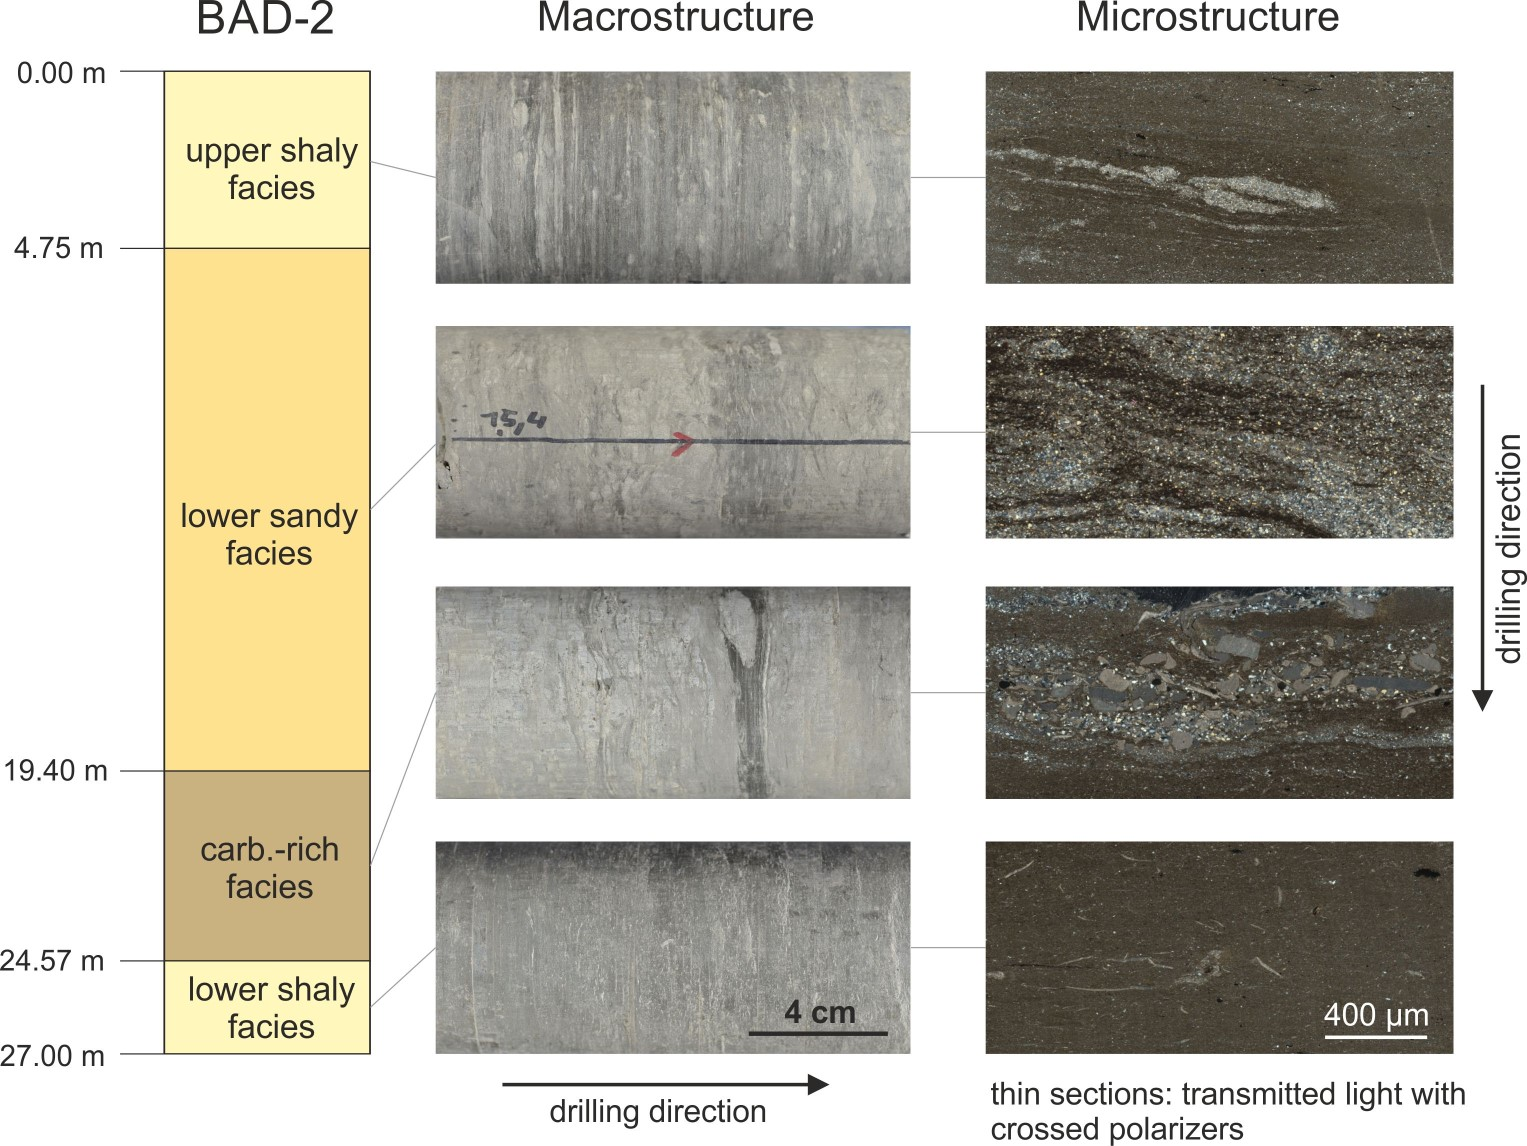
\includegraphics[width=1\textwidth]{./figures/bgr_AD_experiment.jpg}
\caption{Schematic profile of borehole BAD-2 as marked in Figure \ref{fig:bgr_mt_topview} (left), macrostructural (on drillcore scale) and microstructural features (on thin section scale) of the different facies types of Opalinus Clay encountered in the BAD-2 borehole.}
\label{fig:bgr_AD_experiment}
\end{figure}